\documentclass{standalone}
\usepackage{tikz}
\usetikzlibrary{patterns, positioning}
\usepackage[sfdefault]{ClearSans} %% option 'sfdefault' activates Clear Sans as the default text font
\usepackage[T1]{fontenc}

\begin{document}
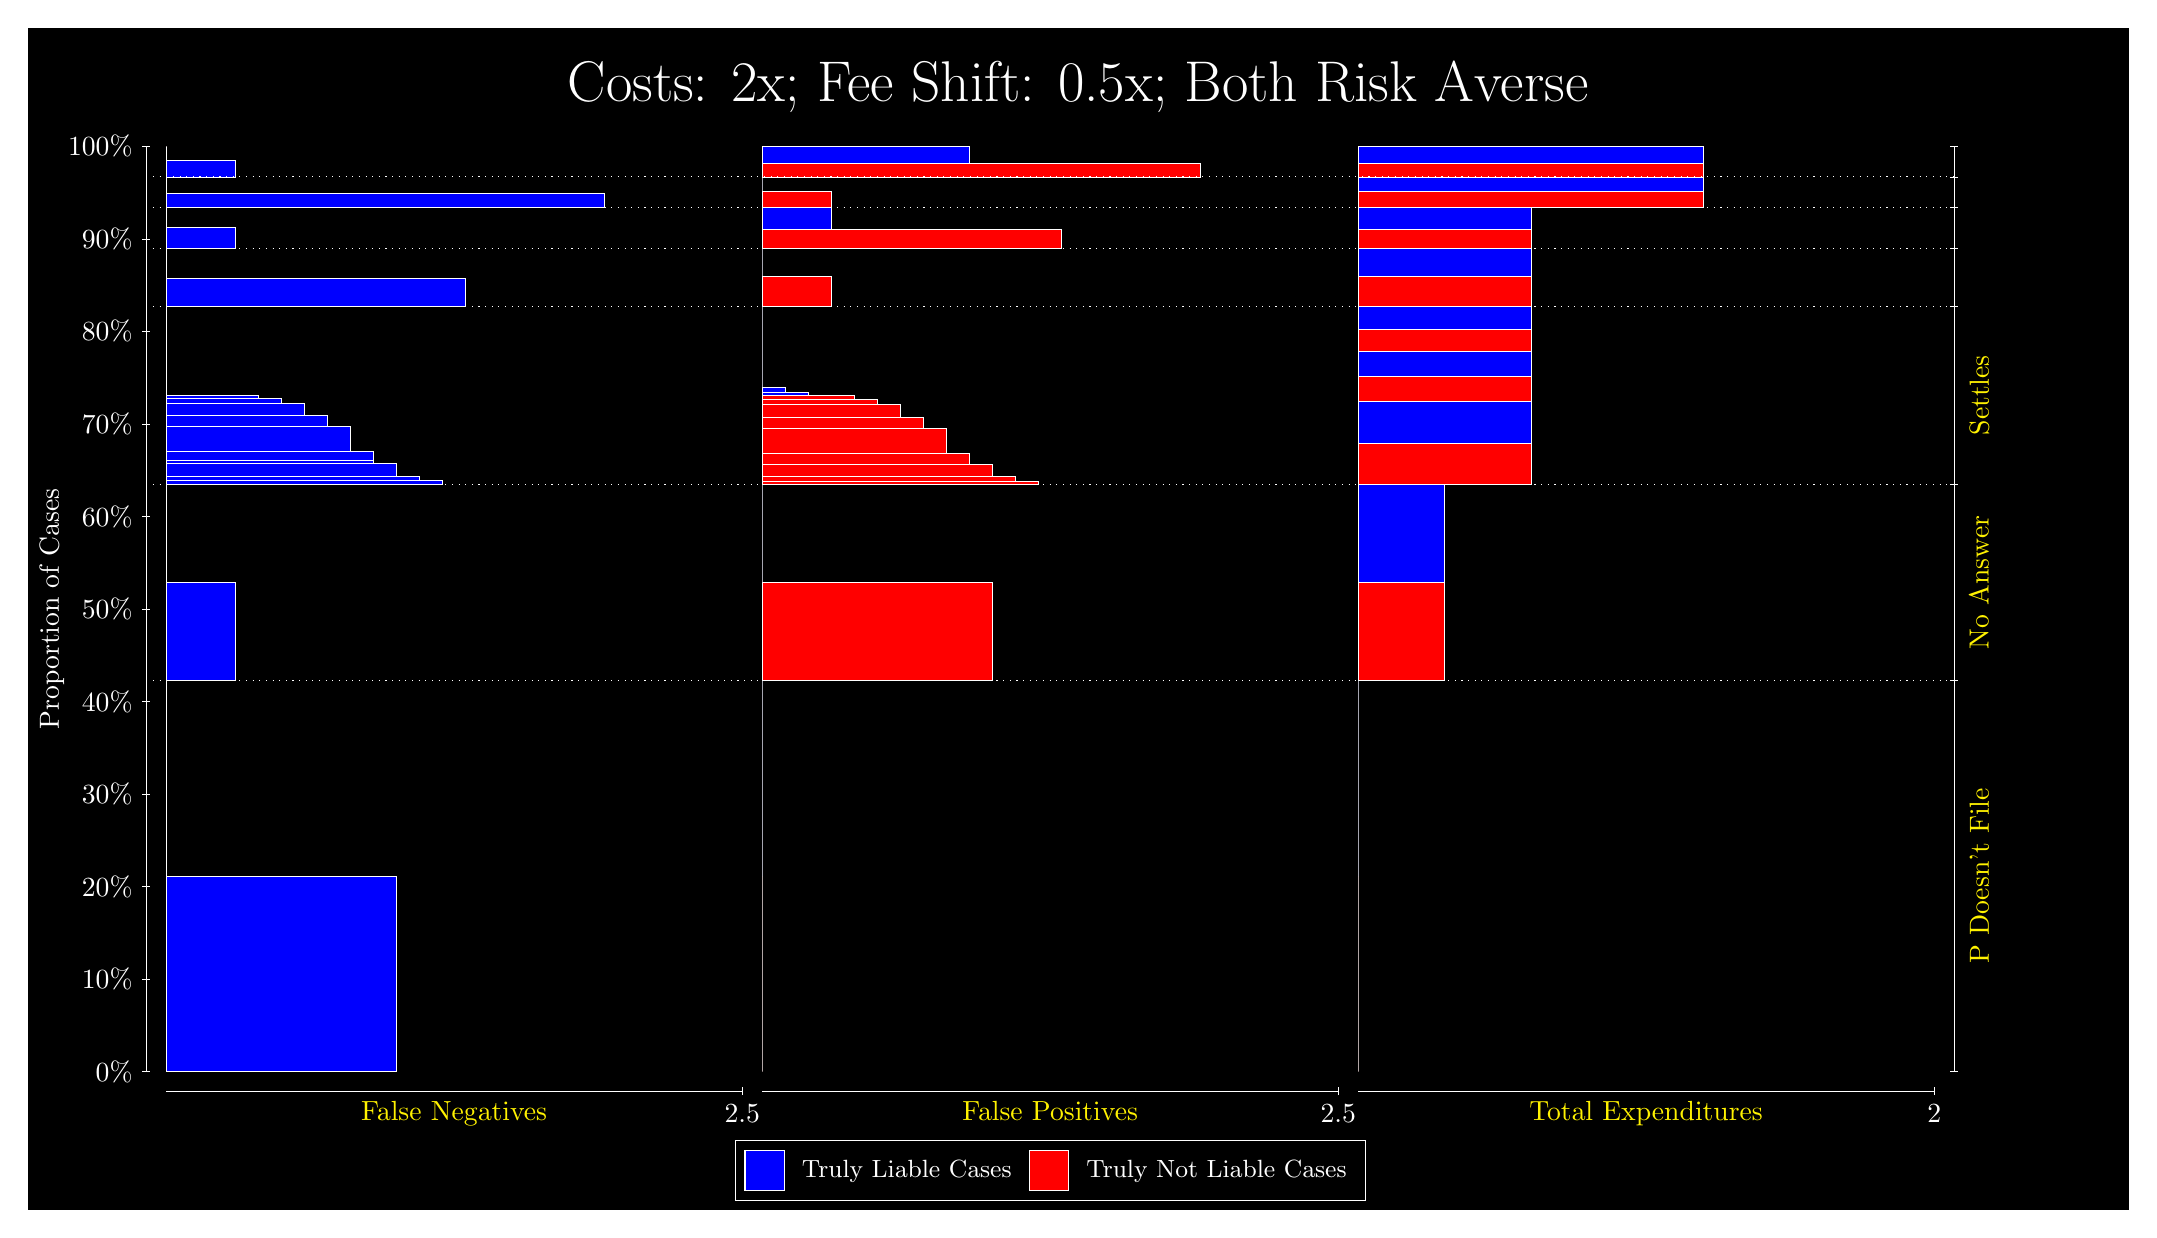
\begin{tikzpicture}
\draw[fill=black] (0,0) rectangle (26.667,15);
\draw[text=white] (0,13.5) rectangle (26.667,15) node[midway] {\huge Costs: 2x; Fee Shift: 0.5x; Both Risk Averse};
\draw[white, very thin] (1.5,1.75) -- (1.5,13.5);
\node[rotate=90, text=white, anchor=center] at (0.3, 7.625) {Proportion of Cases};
\draw[white, very thin] (1.45,1.75) -- (1.55,1.75);
\node[text=white, anchor=east] at (1.45, 1.75) {0\%};
\draw[white, very thin] (1.45,2.925) -- (1.55,2.925);
\node[text=white, anchor=east] at (1.45, 2.925) {10\%};
\draw[white, very thin] (1.45,4.1) -- (1.55,4.1);
\node[text=white, anchor=east] at (1.45, 4.1) {20\%};
\draw[white, very thin] (1.45,5.275) -- (1.55,5.275);
\node[text=white, anchor=east] at (1.45, 5.275) {30\%};
\draw[white, very thin] (1.45,6.45) -- (1.55,6.45);
\node[text=white, anchor=east] at (1.45, 6.45) {40\%};
\draw[white, very thin] (1.45,7.625) -- (1.55,7.625);
\node[text=white, anchor=east] at (1.45, 7.625) {50\%};
\draw[white, very thin] (1.45,8.8) -- (1.55,8.8);
\node[text=white, anchor=east] at (1.45, 8.8) {60\%};
\draw[white, very thin] (1.45,9.975) -- (1.55,9.975);
\node[text=white, anchor=east] at (1.45, 9.975) {70\%};
\draw[white, very thin] (1.45,11.15) -- (1.55,11.15);
\node[text=white, anchor=east] at (1.45, 11.15) {80\%};
\draw[white, very thin] (1.45,12.325) -- (1.55,12.325);
\node[text=white, anchor=east] at (1.45, 12.325) {90\%};
\draw[white, very thin] (1.45,13.5) -- (1.55,13.5);
\node[text=white, anchor=east] at (1.45, 13.5) {100\%};

\draw[white, very thin] (24.457,1.75) -- (24.457,13.5);
\draw[white, very thin] (24.407,1.75) -- (24.507,1.75);
\node[anchor=west] at (24.407, 1.75) {};
\draw[white, very thin] (24.407,6.7144) -- (24.507,6.7144);
\node[anchor=west] at (24.407, 6.7144) {};
\draw[white, very thin] (24.407,9.2077) -- (24.507,9.2077);
\node[anchor=west] at (24.407, 9.2077) {};
\draw[white, very thin] (24.407,11.471) -- (24.507,11.471);
\node[anchor=west] at (24.407, 11.471) {};
\draw[white, very thin] (24.407,12.199) -- (24.507,12.199);
\node[anchor=west] at (24.407, 12.199) {};
\draw[white, very thin] (24.407,12.728) -- (24.507,12.728);
\node[anchor=west] at (24.407, 12.728) {};
\draw[white, very thin] (24.407,13.113) -- (24.507,13.113);
\node[anchor=west] at (24.407, 13.113) {};
\draw[white, very thin] (24.407,13.5) -- (24.507,13.5);
\node[anchor=west] at (24.407, 13.5) {};

\draw[white, very thin, fill=blue] (1.75,1.75) rectangle (4.6775,4.2322);
\draw[white, very thin, fill=red] (1.75,4.2322) rectangle (1.75,6.7144);
\draw[white, very thin, fill=blue] (1.75,6.7144) rectangle (2.6283,7.961);
\draw[white, very thin, fill=red] (1.75,7.961) rectangle (1.75,9.2077);
\draw[white, very thin, fill=blue] (1.75,9.2077) rectangle (5.2631,9.2581);
\draw[white, very thin, fill=blue] (1.75,9.2581) rectangle (4.9703,9.3141);
\draw[white, very thin, fill=blue] (1.75,9.3141) rectangle (4.6775,9.4747);
\draw[white, very thin, fill=blue] (1.75,9.4747) rectangle (4.3848,9.5165);
\draw[white, very thin, fill=blue] (1.75,9.5165) rectangle (4.3848,9.6256);
\draw[white, very thin, fill=blue] (1.75,9.6256) rectangle (4.092,9.9453);
\draw[white, very thin, fill=blue] (1.75,9.9453) rectangle (3.7993,10.083);
\draw[white, very thin, fill=blue] (1.75,10.083) rectangle (3.5065,10.238);
\draw[white, very thin, fill=blue] (1.75,10.238) rectangle (3.2138,10.297);
\draw[white, very thin, fill=blue] (1.75,10.297) rectangle (2.921,10.341);
\draw[white, very thin, fill=red] (1.75,10.341) rectangle (1.75,11.471);
\draw[white, very thin, fill=blue] (1.75,11.471) rectangle (5.5558,11.819);
\draw[white, very thin, fill=red] (1.75,11.819) rectangle (1.75,12.199);
\draw[white, very thin, fill=blue] (1.75,12.199) rectangle (2.6283,12.475);
\draw[white, very thin, fill=red] (1.75,12.475) rectangle (1.75,12.728);
\draw[white, very thin, fill=blue] (1.75,12.728) rectangle (7.3123,12.906);
\draw[white, very thin, fill=red] (1.75,12.906) rectangle (1.75,13.113);
\draw[white, very thin, fill=blue] (1.75,13.113) rectangle (2.6283,13.324);
\draw[white, very thin, fill=red] (1.75,13.324) rectangle (1.75,13.5);
\draw[white, very thin, fill=red] (9.3189,1.75) rectangle (9.3189,4.2322);
\draw[white, very thin, fill=blue] (9.3189,4.2322) rectangle (9.3189,6.7144);
\draw[white, very thin, fill=red] (9.3189,6.7144) rectangle (12.246,7.961);
\draw[white, very thin, fill=blue] (9.3189,7.961) rectangle (9.3189,9.2077);
\draw[white, very thin, fill=red] (9.3189,9.2077) rectangle (12.832,9.2498);
\draw[white, very thin, fill=red] (9.3189,9.2498) rectangle (12.539,9.3068);
\draw[white, very thin, fill=red] (9.3189,9.3068) rectangle (12.246,9.4591);
\draw[white, very thin, fill=red] (9.3189,9.4591) rectangle (11.954,9.5966);
\draw[white, very thin, fill=red] (9.3189,9.5966) rectangle (11.661,9.9145);
\draw[white, very thin, fill=red] (9.3189,9.9145) rectangle (11.368,10.065);
\draw[white, very thin, fill=red] (9.3189,10.065) rectangle (11.075,10.227);
\draw[white, very thin, fill=red] (9.3189,10.227) rectangle (10.783,10.285);
\draw[white, very thin, fill=red] (9.3189,10.285) rectangle (10.49,10.337);
\draw[white, very thin, fill=blue] (9.3189,10.337) rectangle (9.9044,10.382);
\draw[white, very thin, fill=blue] (9.3189,10.382) rectangle (9.6116,10.441);
\draw[white, very thin, fill=blue] (9.3189,10.441) rectangle (9.3189,11.471);
\draw[white, very thin, fill=red] (9.3189,11.471) rectangle (10.197,11.851);
\draw[white, very thin, fill=blue] (9.3189,11.851) rectangle (9.3189,12.199);
\draw[white, very thin, fill=red] (9.3189,12.199) rectangle (13.125,12.451);
\draw[white, very thin, fill=blue] (9.3189,12.451) rectangle (10.197,12.728);
\draw[white, very thin, fill=red] (9.3189,12.728) rectangle (10.197,12.935);
\draw[white, very thin, fill=blue] (9.3189,12.935) rectangle (9.3189,13.113);
\draw[white, very thin, fill=red] (9.3189,13.113) rectangle (14.881,13.29);
\draw[white, very thin, fill=blue] (9.3189,13.29) rectangle (11.954,13.5);
\draw[white, very thin, fill=red] (16.888,1.75) rectangle (16.888,4.2322);
\draw[white, very thin, fill=blue] (16.888,4.2322) rectangle (16.888,6.7144);
\draw[white, very thin, fill=red] (16.888,6.7144) rectangle (17.986,7.961);
\draw[white, very thin, fill=blue] (16.888,7.961) rectangle (17.986,9.2077);
\draw[white, very thin, fill=red] (16.888,9.2077) rectangle (19.083,9.7349);
\draw[white, very thin, fill=blue] (16.888,9.7349) rectangle (19.083,10.268);
\draw[white, very thin, fill=red] (16.888,10.268) rectangle (19.083,10.582);
\draw[white, very thin, fill=blue] (16.888,10.582) rectangle (19.083,10.891);
\draw[white, very thin, fill=red] (16.888,10.891) rectangle (19.083,11.179);
\draw[white, very thin, fill=blue] (16.888,11.179) rectangle (19.083,11.471);
\draw[white, very thin, fill=red] (16.888,11.471) rectangle (19.083,11.851);
\draw[white, very thin, fill=blue] (16.888,11.851) rectangle (19.083,12.199);
\draw[white, very thin, fill=red] (16.888,12.199) rectangle (19.083,12.451);
\draw[white, very thin, fill=blue] (16.888,12.451) rectangle (19.083,12.728);
\draw[white, very thin, fill=red] (16.888,12.728) rectangle (21.279,12.935);
\draw[white, very thin, fill=blue] (16.888,12.935) rectangle (21.279,13.113);
\draw[white, very thin, fill=red] (16.888,13.113) rectangle (21.279,13.29);
\draw[white, very thin, fill=blue] (16.888,13.29) rectangle (21.279,13.5);
\draw[white, dotted] (1.5,6.7144) -- (24.457,6.7144);
\draw[white, dotted] (1.5,9.2077) -- (24.457,9.2077);
\draw[white, dotted] (1.5,11.471) -- (24.457,11.471);
\draw[white, dotted] (1.5,12.199) -- (24.457,12.199);
\draw[white, dotted] (1.5,12.728) -- (24.457,12.728);
\draw[white, dotted] (1.5,13.113) -- (24.457,13.113);
\draw[white, very thin] (1.75,1.5) -- (9.0689,1.5);
\node[text=yellow, anchor=north] at (5.4094, 1.5) {False Negatives};
\draw[white, very thin] (9.0689,1.45) -- (9.0689,1.55);
\node[text=white, anchor=north] at (9.0689, 1.45) {2.5};

\draw[white, very thin] (9.3189,1.5) -- (16.638,1.5);
\node[text=yellow, anchor=north] at (12.978, 1.5) {False Positives};
\draw[white, very thin] (16.638,1.45) -- (16.638,1.55);
\node[text=white, anchor=north] at (16.638, 1.45) {2.5};

\draw[white, very thin] (16.888,1.5) -- (24.207,1.5);
\node[text=yellow, anchor=north] at (20.547, 1.5) {Total Expenditures};
\draw[white, very thin] (24.207,1.45) -- (24.207,1.55);
\node[text=white, anchor=north] at (24.207, 1.45) {2};

\node[text=yellow, centered, rotate=90] at (24.777, 4.2322) {P Doesn't File};
\node[text=yellow, centered, rotate=90] at (24.777, 7.961) {No Answer};
\node[text=yellow, centered, rotate=90] at (24.777, 10.339) {Settles};





\draw (12.978300999999998,1.5) node[draw=none] (baseCoordinate) {};
\begin{scope}[align=center]
        \matrix[scale=0.5, draw=white, below=0.5cm of baseCoordinate, nodes={draw}, column sep=0.1cm]{
            \node[rectangle, draw, minimum width=0.5cm, minimum height=0.5cm, fill=blue] {}; &
            \node[draw=none, font=\small, text=white] (B) {Truly Liable Cases}; &
            \node[rectangle, draw, minimum width=0.5cm, minimum height=0.5cm, fill=red] {}; &
            \node[draw=none, font=\small, text=white] (B) {Truly Not Liable Cases}; \\
            };
\end{scope}

\end{tikzpicture}
\end{document}